\documentclass{webofc}
\usepackage[varg]{txfonts}   % Web of Conferences font

\usepackage[T2A]{fontenc} % указывает внутреннюю кодировку TeX
\usepackage[english]{babel}   %% загружает пакет многоязыковой вёрстки
\usepackage{color}
\usepackage{tasks}
\settasks {counter-format=(tsk[r])}
%\usepackage{exsheets}
\usepackage{array,graphicx,caption,paralist}
\usepackage{floatflt,wrapfig}
\newcommand{\er}{\textmd{EXPERTroot}}

\begin{document}
\title{Timing properties of the NeuRad detector}

\author{\firstname{I.} \lastname{Muzalevsky}\inst{1,2,3}\fnsep\thanks{\email{ivanmuzalevskij@gmail.com}} \and
	\firstname{V.} \lastname{Chudoba}\inst{1,2}\fnsep\thanks{\email{chudoba@jinr.ru}} \and
	\firstname{A.} \lastname{Bezbakh}\inst{1,2} \and
	\firstname{S.} \lastname{Belogurov}\inst{1} \and
	\firstname{I.} \lastname{Mukha}\inst{4} \and
	\firstname{O.} \lastname{Kiselev}\inst{4} \and
	\firstname{A.} \lastname{Fomichev}\inst{1} \and
	\firstname{S.} \lastname{Krupko}\inst{1} \and
	\firstname{R.} \lastname{Slepnev}\inst{1} \and
	\firstname{D.} \lastname{Kostyleva}\inst{4} \and
	\firstname{A.} \lastname{Gorshkov}\inst{1} \ for the EXPERT project.
	% etc.
}
\institute{
	FLNR JINR Dubna, Russia; 
	\and
	Silesian University in Opava, Czech Republic;
	\and
	Dubna State University, Russia;
	\and
	GSI Helmholtzzentrum, Darmstadt
}
\abstract{%
%	\color{red}
	One of the subtopics of the SuperFRS Experiment Collaboration, being part of NUSTAR@FAIR, is investigation of properties of light exotic nuclei using EXPERT setup.
	One of its modules, the NeuRad detector, will be intended for registration of neutrons emitted from investigated nuclei.
	Present work is dedicated to investigation of the timing properties of the NeuRad prototype. 
}
%
\maketitle
%
%\color{red}
\section{Introduction}
Properties of exotic nuclei represent one of the most important fields in modern nuclear physics.
Such uncommon nuclei are characterized by large excess of neutrons or protons and are located far from the line of nuclear stability. As far as binding energy decreases, one may observe the transition from the discrete spectra to nuclear resonances with many overlapping states and, as a consequence, such phenomena as neutron halo, soft mode of dipole excitation and others could be observed. Moreover, new decay channels, including many-body, are becoming open.

As far as exotic nuclei are unstable one meet a problem how to produce them.
One of the most developed facility for their production by separation in-flight will be fragment separator Super-FRS at FAIR (Facility for Antiproton and Ion Research) \cite{diplom}. Project EXPERT (EXotic Particle Emission and Radioactivity by Tracking \cite{IMexpert}) dedicated to study of properties of exotic nuclei is a part of program of the Super-FRS Experiment Collaboration. EXPERT setup consists of five modules each of which is intended to detect different decay products.
These modules may be enumerated as:
\begin{inparaenum}[(i)]
	\item Radiation-hard silicon strip detector (SSD).
	\item Microstrip silicon ($\mu$Si) tracking detectors.
	\item The gamma-ray and light particles detector system GADAST (GAmma-ray Detectors Around Secondary Target).
	\item The OTPC (Optical Time Projection Chamber) for radioactivity studies by the implantation-decay method.
	\item The NeuRad (Neutron Radioactivity) fine-resolution detector of neutrons.
\end{inparaenum}

Additional important part of the EXPERT project is a framework for simulations of the experiments and processing of the experimental data. For this purpose a framework EXPERTroot \cite{er} has been developed.
%EXPERTroot is a framework for Monte-Carlo simulations of detector responses, event reconstruction and EXPERT experiment analysis.
This paper is dedicated to exploration of the NeuRad timing properties obtained in tests of the NeuRad prototype. All necessary methods of data processing and simulation were implemented into the EXPERTroot.

\section{Test of NeuRad timing properties}
Neutron detector NeuRad is aimed at providing precise information on angular correlations between nuclear-decay neutrons emitted from decay and heavy ion fragment which will be identified by Super-FRS beam diagnostic system. An information on angular correlations will be used to determine decay energy of the precursor and its lifetime. Trajectories of a heavy ion and neutrons will be reconstructed by an array of the $\mu$Si detectors and the NeuRad detector respectively. %The trajectories of neutrons will be reconstructed from the data obtained by NeuRad.  %This number is determined by the low transfer momentum of the decay with energies expected in the range of 0.1-100 keV.  
NeuRad will be constructed from a large number of scintillating fibers ($\approx$10000 units). Each fiber will have a square cross section of 3$\times$3\,mm$^2$ and the length of 1\,m. Scintillating fibers will be grouped into bundles. 
The neutrons penetrating into the bundles will be mostly elastically scattered on protons (approximately 10\% of neutrons will be scattered on the carbon nuclei). In such case recoil proton will induce a scintillation flash inside the fiber. The light emitted within the full reflection angle travels to the multi-anode photomultiplier tubes (MAPMT) located at the both ends of the fiber.
MAPMT's will be mounted to the bundles so that the area of each pixel corresponding to its anode will completely overlap the frontal surface of one fiber.

\begin{figure}[h]
	\center{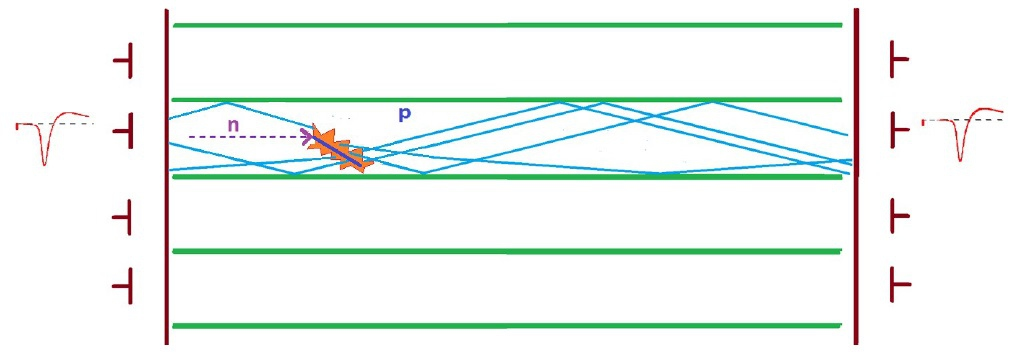
\includegraphics[width=1\linewidth]{neurad.png}}
	\caption{Illustration of the operational principle of the NeuRad detector. Each scintillating fiber will be coupled to one anode of the MAPMT. The neutron beam will penetrate through the frontal MAPMT's.}
	\label{ris:neuradPrinciple}
\end{figure}

In the course of planned experiments, NeuRad will be placed in 28 meters downstream of the secondary target so that the fibers will be oriented along the beam direction, see Fig.\ref{ris:neuradPrinciple}.
This is planned in order to provide sufficient efficiency of the detection and fine position resolution for neutrons with energies between 200 and 800\,MeV in laboratory system.
With such a configuration the total angular acceptance of the detector will be about 12\,mrad.
Thus, the neutron beam will pass through the photomultiplier tubes before penetrating into the sensitive scintillating material.
Two coordinates, transverse to the direction of the beam, of the neutron interaction with the scintillating material will be obtained from the number of the fired fibers in which the scattering would be occurred.
The longitudinal coordinate will be determined from measurement of the time difference of the signals from two MAPT's located on the opposite sides of the detector.
The accuracy of determining the longitudinal coordinate of the interaction depends on time resolution of the detector which is one of the significant characteristics of the intended NeuRad device.
%Time resolution is the accuracy of determining the time of interaction of a particle with the detector	.
For example, in order to obtain 20\,cm position resolution one has to ensure time-uncertainty better than 1\,ns.
Also it is important to determine exactly the first neutron hit and following sequence of the signals induced in the detector material. This information allows to distinguish multi-neutron events from the multiple hits of a single re-scattered neutron.

%\section{Measurements}

The first investigation aimed to obtain timing characteristics of the NeuRad detector was conducted recently in Flerov Laboratory of Nuclear Reactions JINR, Dubna. The NeuRad prototype was used for these test measurements. The sensitive part of the prototype was a bundle of 256 optical fibers made of scintillator plastic BCF-12 \cite{crystals}. Each fiber was  3$\times$3\,mm$^2$ in cross section and 25\,cm long.
Two MAPMT's Hamamatsu9500 (H9500) \cite{hm} were mounted to both sides of the bundle.


\begin{figure}[h]
	\centering
	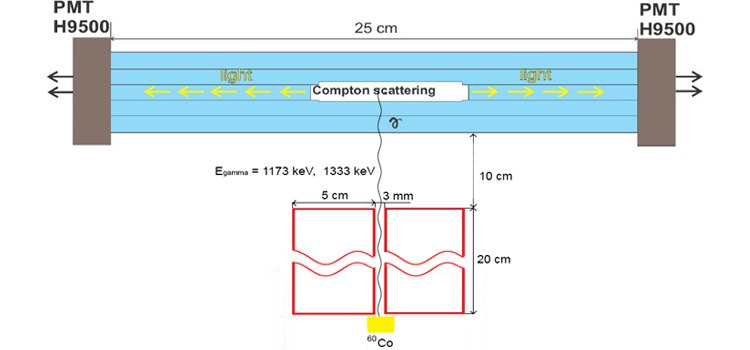
\includegraphics[width=1\linewidth]{NeuRadexperiment.png}
	\captionof{figure}{NeuRad measurements scheme. The prototype was irradiated by standart gamma source $^{60}$Co. The beam was focused at the geometrical center of the bundle and signals were collected by couple of H9500 MAPMT's.}
	\label{ris:neuradexp}
\end{figure}

This prototype was irradiated by collimated gamma beam with energies $E^{(1)}_{\gamma}$=1173\,keV and $E^{(2)}_{\gamma}$=1333\,keV emitted by $^{60}$Co as showed in Fig.~\ref{ris:neuradexp}. The beam was focused at the geometrical center of the prototype. Signals obtained from MAPMT's was collected by the Tektronix oscilloscope MSO7354 and DRS4 evaluation board and their form were saved for each detected event.

\section{Simulations and data processing in EXPERTroot}

All conducted measurements were simulated in the \er. For all simulations in \er\, method of simulating detector response \cite{er} is used.
Formation of a virtual model of the setup described above was the first step.
%	The \er\, options allow to create any shape of detector model and fill in with any material.	RNF grant, LM and LTT grant, ICRF?
Virtual model of the experimental setup is showed in Fig.\ref{ris:sim}a). 
	
	\begin{figure} 
		\begin{minipage}[h]{\linewidth} 
			\center{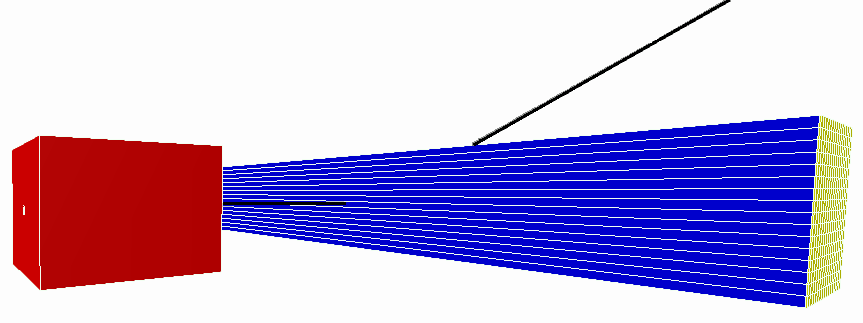
\includegraphics[width=0.9\linewidth]{sim.png}} a) \\ 
		\end{minipage} 
		\vfill 
		\begin{minipage}[h]{0.47\linewidth} 
			\center{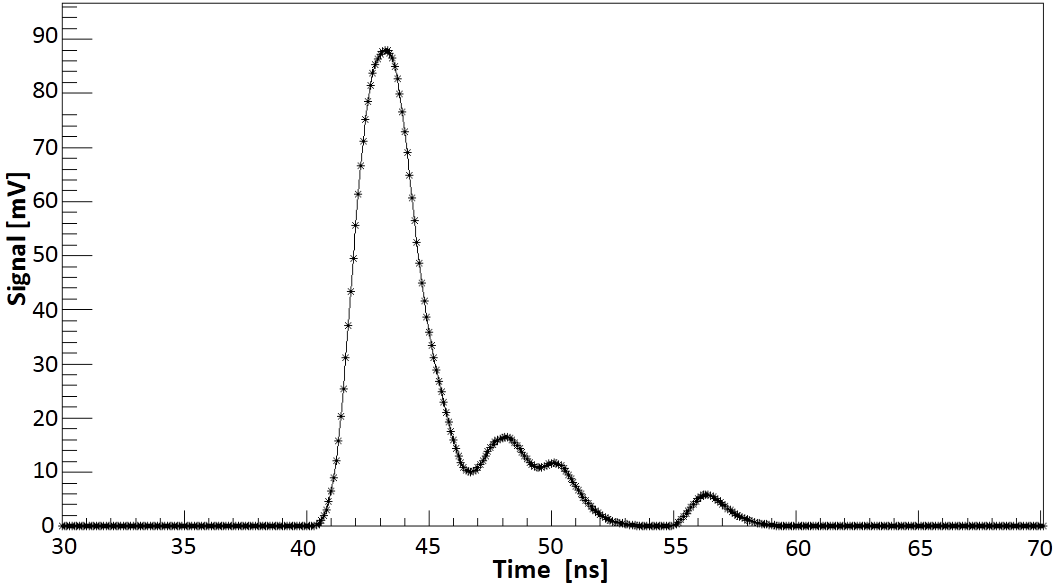
\includegraphics[width=1\linewidth]{simSignal1.png}} b) \\
		\end{minipage} 
		\hfill 
		\begin{minipage}[h]{0.47\linewidth} 
			\center{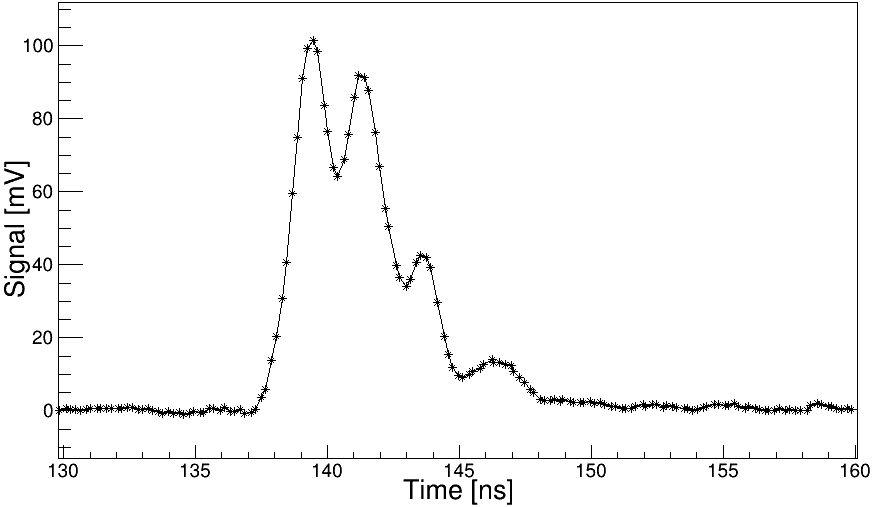
\includegraphics[width=1\linewidth]{originalsignalform.png}} c) \\ 
		\end{minipage} 
		\caption{a) Simulations in \er. Bundle and collimator are depicted in blue, red colors respectively. The trajectory of the gamma particle is colored in black. b) Typical MAPMT's anode output signal form obtained in simulations c) Typical signal form obtained in measurements.} 
		\label{ris:sim} 
	\end{figure}
Then, the transportation of the particles through the volume of the detector was occurred and energy deposits of tracked particles at each step were saved.
This procedure was performed using GEANT4 \cite{geant4} methods. Afterwards, the energy deposits were converted into detector responses having identical format with experimental data.
In order to obtain plausible data all major physical effects which were occurring in the experiment except electronics noise were taken into account in simulations.
Detector characteristics such as de-excitation scintillator time, quantum efficiency of the photocathode, the amplitude oAcknoledgementf the single electron signal, and others were parametrized in simulations and fitted by analysis of the experimental data.
	% or taken from used devices documentation.
	%For simulations the conducted measurements method of simulation of the detector response \cite{diplom} was used. 
The MAPMT anode signal was calculated as a sum of the single photoelectron signals.
The above describe simulation allowed us to save the signal shapes  from all MAPMT anodes in the selected event.
Typical signal forms obtained in simulations and measurements turned out similar and are shown in Fig.\ref{ris:sim}b) and Fig.\ref{ris:sim}c) respectively.
	
The \er\, was used for processing of the obtained data as well.
Several methods of the data processing were developed and implemented into the \er, for example well-known methods of obtaining signal time Constant Fraction Discriminator (CFD) and Leading Edge Discriminator (LED) \cite{diplom}.
%	The main advantage of using \er\, for data processing is a possibility to add any new processing algorithms to the framework at any time.
	Implemented algorithms allowed us to get such time-to-amplitude properties of the signal as rising time, Time-over-Threshold (ToT), anode charge and others. 
%	Methods of the \er\, allowed to get data from simulations of the same format as in experiment. That's why the same algorithms were used for simulation and experimental data.
%	\color{red}
%	As the gamma beam was collimated 

\begin{wrapfigure}{l}{0.5\linewidth}
	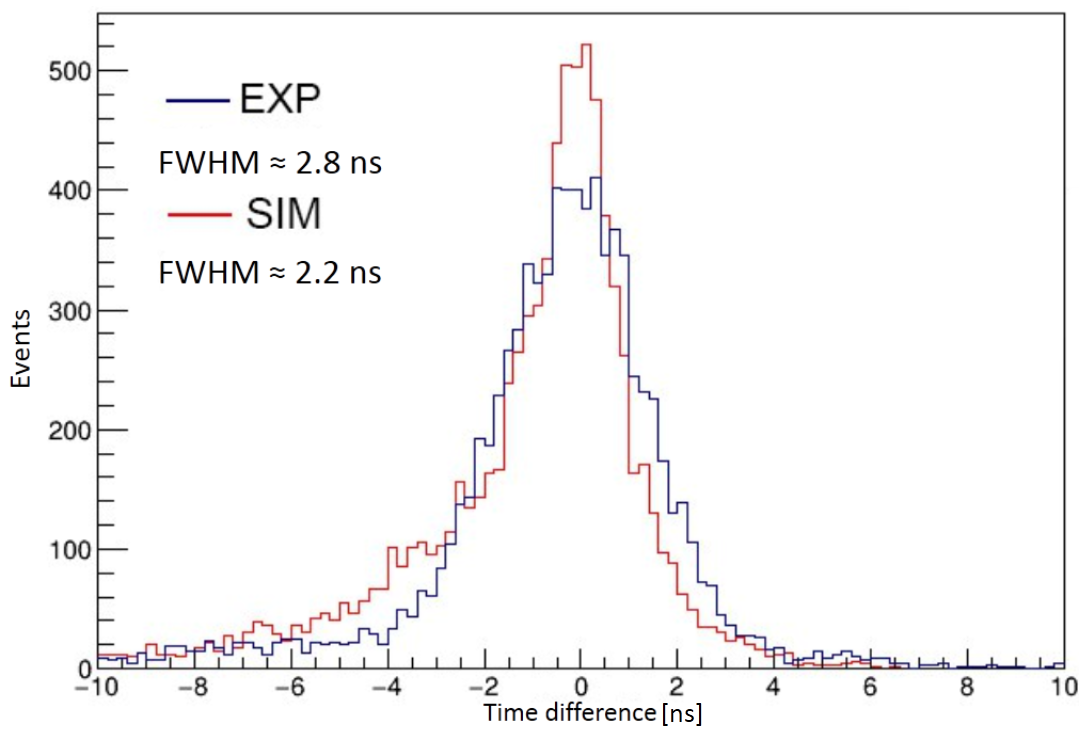
\includegraphics[width=\linewidth]{tausim.png}
	\caption{The time difference distribution for experimental (blue) and simulation data (red). For obtaining time of the signal the LED method was used.}\label{ris:tausim}
\end{wrapfigure}
	
The time resolution of the detector prototype was calculated as a Full Width at Half Maximum (FWHM) of the distribution of the $\Delta \tau$, (difference of collected times from the opposite sides of the selected fiber in the selected event).
%	\color{black}
%
%\section{Results}
%


Taking into account the irregular form of the signals, the most successful method for calculation of the time resolution was LED combined with selection selection  by ToT.
The distribution of the $\Delta \tau$ values is showed in Fig.\ref{ris:tausim}, where experimental and simulated data are depicted by blue and red color, respectively.
The obtained time resolution of the NeuRad prototype is 2.8\,ns for experimental data. It corresponds to accuracy of the longitudinal coordinate determination approximately 56\,cm. For simulations the accuracy of time and the longitudinal determination is 2.2\,ns and 44\,cm respectively.


	
%	\begin{figure}[h]
%		\centering
%		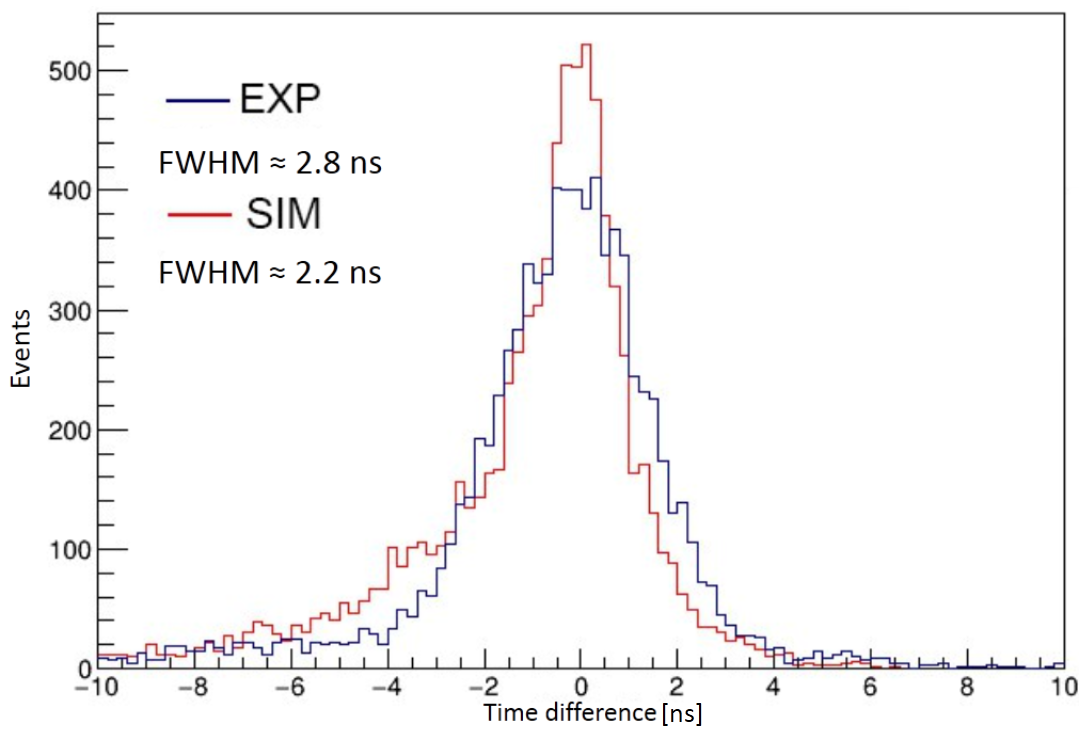
\includegraphics[width=0.8\linewidth]{tausim.png}
%		\caption{The time difference distribution for experimental (blue) and simulation data (red). For obtaining time of the signal the leading edge algorithm was used.}\label{ris:tausim}
%	\end{figure}
	
	
%Fig.\ref{ris:ampsim} shows the amplitude-time correlations for the simulated and experimental data at the left and right parts respectively.

%begin{figure}	RNF grant, LM and LTT grant, ICRF?
%	\centering
%	\includegraphics[width=\linewidth]{ampsim.png}
%	\caption{Зависимость $\Delta\tau$ рассчитанное методом дискриминатора переднего фронта от заряда. Слева для моделированных, справа для экспериментальных данных }\label{ris:ampsim}
%\end{figure}

\section{Conclusion}
	
	Prototype of the NeuRad detector was investigated for the timing properties.
	Standard algorithms for signal processing were implemented into the \er\ framework. The simulation of the MAPMT's time response was developed and implemented as well.
	
%	The time resolution of the prototype turned out to be 2.8\,ns which corresponds to 56\,cm of coordinate resolution.
	
%	All measurements were simulated using \er.
	It was found that the results of experiment and simulation are in a good agreement and it was confirmed that the \er\ options allow to identify the most important effects affecting the timing properties of the intended NeuRad detector.
	Therefore, the results of this work are very important contribution to the development of the EXPERT project.
	
\section{Acknowledgement}
This  work was partly supported by Helmholtz Association under grant agreement IK-RU-002, RSF 17-12-01367 grant and MEYS Projects (Czech Republic) LTT17003 and LM2015049.

	
\begin{thebibliography}{99}
	
	\bibitem{diplom} 
	M. Winkler et al., The status of the Super-FRS in-flight facility at FAIR, Nucl. Instr. and Meth. in Phys. Res. B 266 (2008) 4183.
	
	\bibitem{IMexpert} 
	Geissel, H., Kiselev, O., Mukha, I., et al., "Expert (exotic Particle Emission and Radioactivity by Tracking) Studies at the Super-Frs Spectrometer", 2015, Exotic Nuclei: EXON-2014 - Proceedings of International Symposium.
	
	\bibitem{er}
	http://er.jinr.ru/
	
	\bibitem{hm} 
	www.hamamatsu.com/
	
	\bibitem{crystals} 
	https://www.crystals.saint-gobain.com/
	
	\bibitem{geant4}
	http://geant4.cern.ch/
	
\end{thebibliography}

\end{document}